\chapter{Theorie}
\section{Wie kam es dazu?}

\section{Plötzlicher Kindstod Theorie}
Unter dem Begriff Plötzlicher Kindstod versteht man das Versterben eines Babys welches
das erste Lebensjahr noch nicht vollendet hat und unter keinerlei Vorerkrankungen litt.
Im Zuge der Diagnose muss auch der Fundort des leblosen Kindes untersucht werden um einen Unfalltod, 
durch Ersticken an einer Decke, Kuscheltiers, etc. auszuschließen. 
Deshalb handelt es sich hierbei auch um eine Ausschlussdiagnose. 
In Österreich und anderen Industrienationen der Welt ist SIDS eine der häufigsten diagnostizierten Todesursachen.\cite{meinmed_sids}
Zudem belegen Statistiken, dass der Plötzliche Kindstod vor allem in den Wintermonaten auftritt und meist im Schlaf. \cite{der-ploetzliche-saeuglingstod-epidemiologie-aetiologie-pathophysiologie-und-differenzialdiagnostik} \cite{Poets2020}

\section{Theorie zum allgemeineren System}
%Was kann man zum auslesen von Vitalwerten bzw. unseren Aufnahmedaten so an theorie finden?
%muss nicht wirklich schon genau auf unser System bezogen sein

\section{Was gibt es schon?}
\subsection{Markt}
%KI gesteuerte Babyphone usw.

\subsection{Forschung}
%Babysprachentheorie
%med uni graz Ki Modell

%Bettchen Theorie 

%Roboter Theorie 
\section{Testroboter}
\subsection{BLE und Interface}
\subsubsection{BLE Architektur} 
Bluetooth Low Energy ist eine Bluetooth Protokoll, das im Vergleich zu Classic Bluetooth einen geringeren Stromverbrauch hat und somit auch einen niedrigere Datentransferrate erreicht.
Es wird vor allem im Bereich Internet of Things (IoT) und für Kommunikation mit Messsensoren benutzt.
BLE ist nicht kompatibel mit Classic Bluetooth. 
Das BLE Protokoll ist in drei Schichten geteilt.
\begin{itemize}
\item Application Layer
\item Host Layer
\item und Controller Layer
\item \end{itemize}
siehe Abbildung \ref{fig:ble_architektur}

\begin{figure}[htbp]
\centering
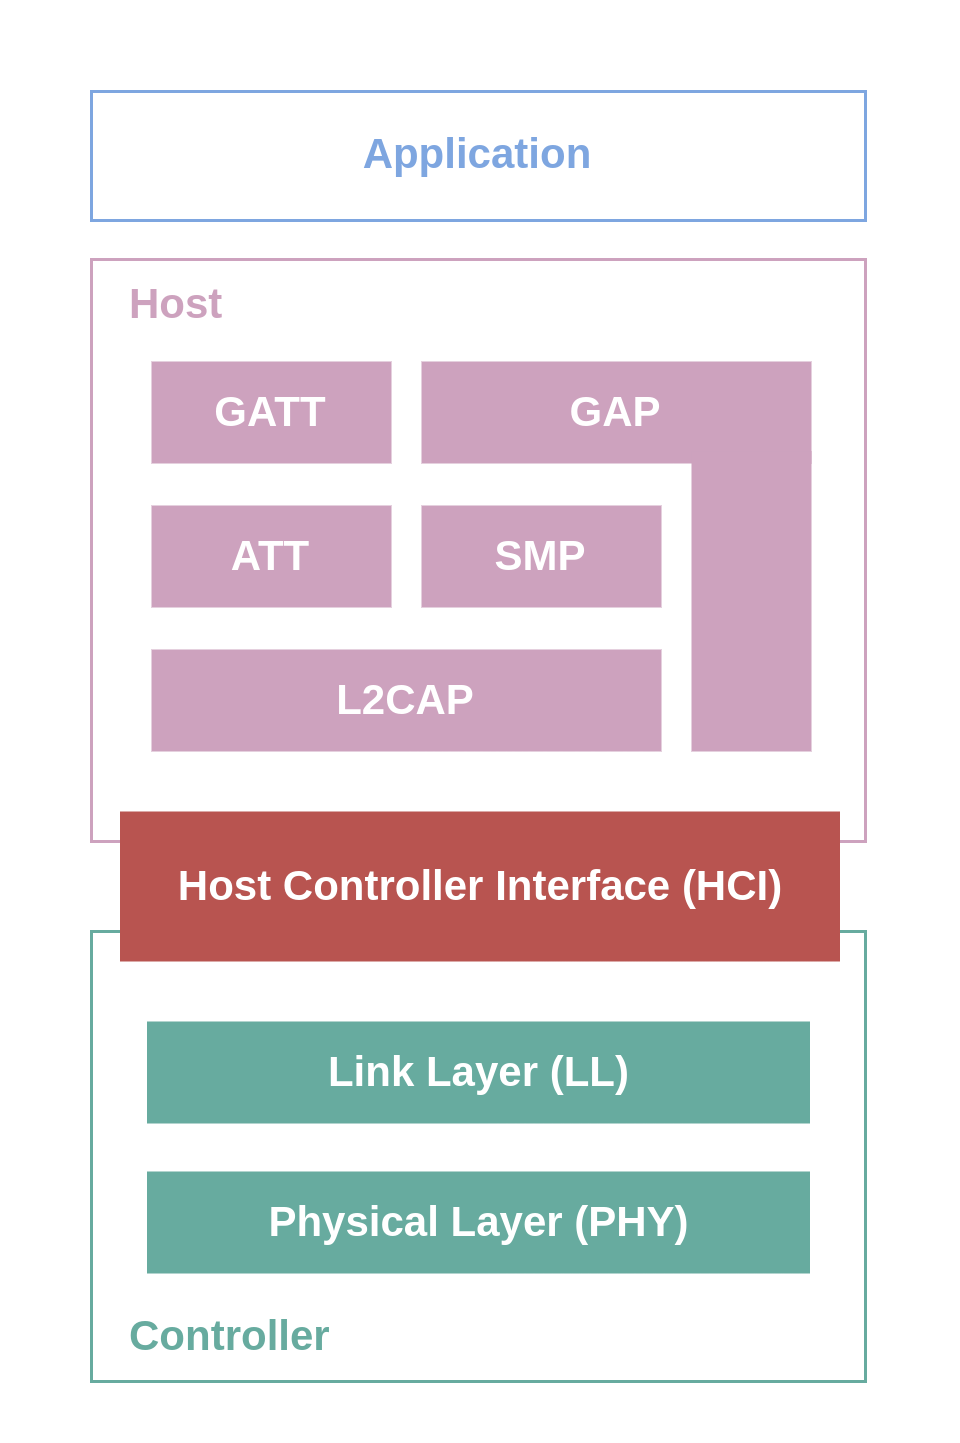
\includegraphics[width=7cm]{images/ble-architecture.png}
\caption{BLE Architektur}
\label{fig:ble_architektur}
\end{figure}

\noindent
In der Application Layer können wir unsere Anwendung mit BLE realisieren. Hier implementiert man seine Anforderungen.In der Host Layer findet die Kommunikation zwischen Benutzeranwendung und Controllinterface der Hardware statt, man nennt diese Ebene auch Host Stack. Der in Kombination mit dem Controller Stack den Bluetooth Stack bildet. Alle relevanten Bluetooth LE Protokolle der Hostseite sind hier implementiert.\cite{espressif_bluetooth_architecture} In der letzten Schicht, der Controller Layer finden die physical und die link Layer ihren Platz. Sie interagieren direkt mit der Hardware. Die BLE-Protokolle der Host Schicht sind GAP, ATT, GATT, SMP und L2CAP.\cite{espressif_ble_intro}
\newpage

\subsubsection{GAP (Generic Accsess Profile)}
Ist für die Verbindung von zwei BLE-Geräten verantwortlich. Das Protokoll ist in 3 verschiedene Modi geteilt je nachdem welcher Verbindungsgrad erfüllt ist. Innerhalb dieser gibt es Rollen die den Geräten zugeteilt sind. 
 
\begin{figure}[h]
\centering
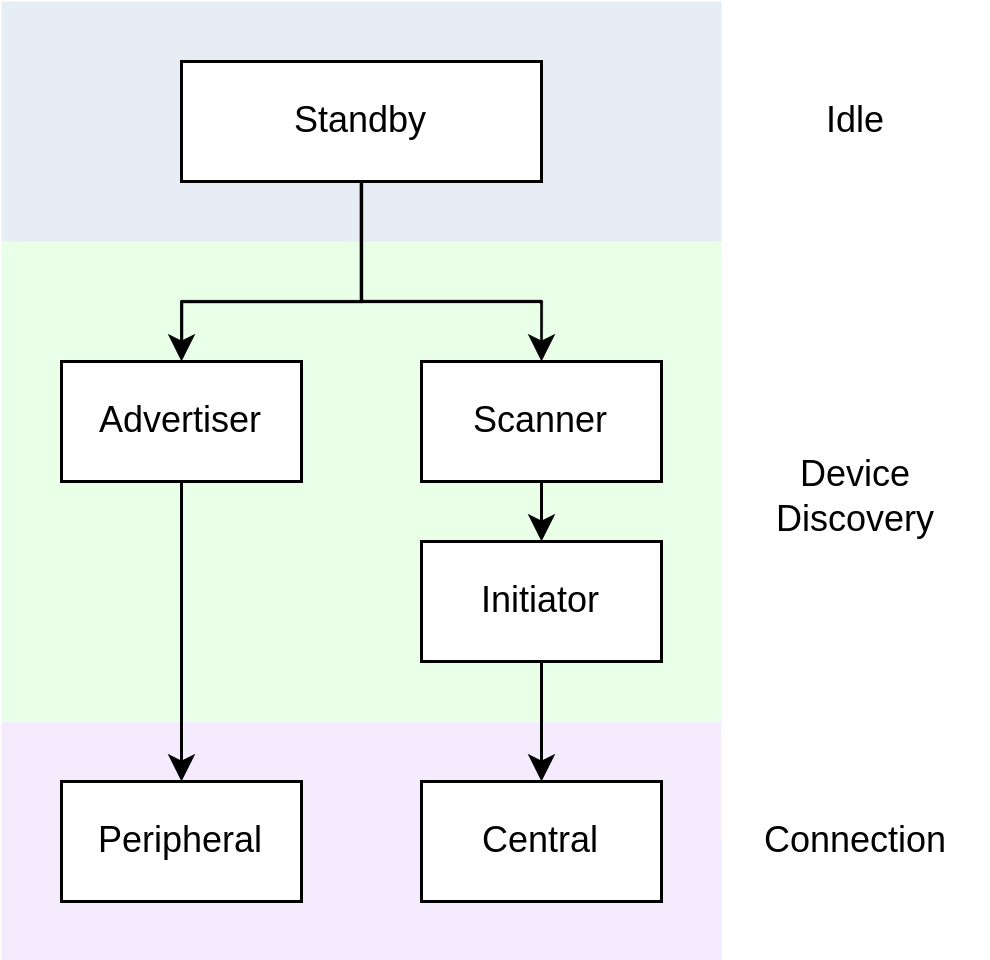
\includegraphics[width = 4cm]{images/ble-gap.png}
\caption{BLE GAP}
\label{fig:ble_gap}
\end{figure}
\noindent
In unserem Projekt übernimmt der ESP32 die Rolle des Servers, und der Laptop ist der Client. 
Im GAP werden diese Rollen mit Peripheral (Server) und Central (Client) bezeichnet. \cite{espressif_ble_intro} Anhand von Abbildung \ref{fig:ble_gap_bsp} lässt sich der Verbindungsaufbau und die unterschiedlichen Rollen welche die Teilnehmener dabei annehmen nachvollziehen.
\begin{figure}[h]
\centering
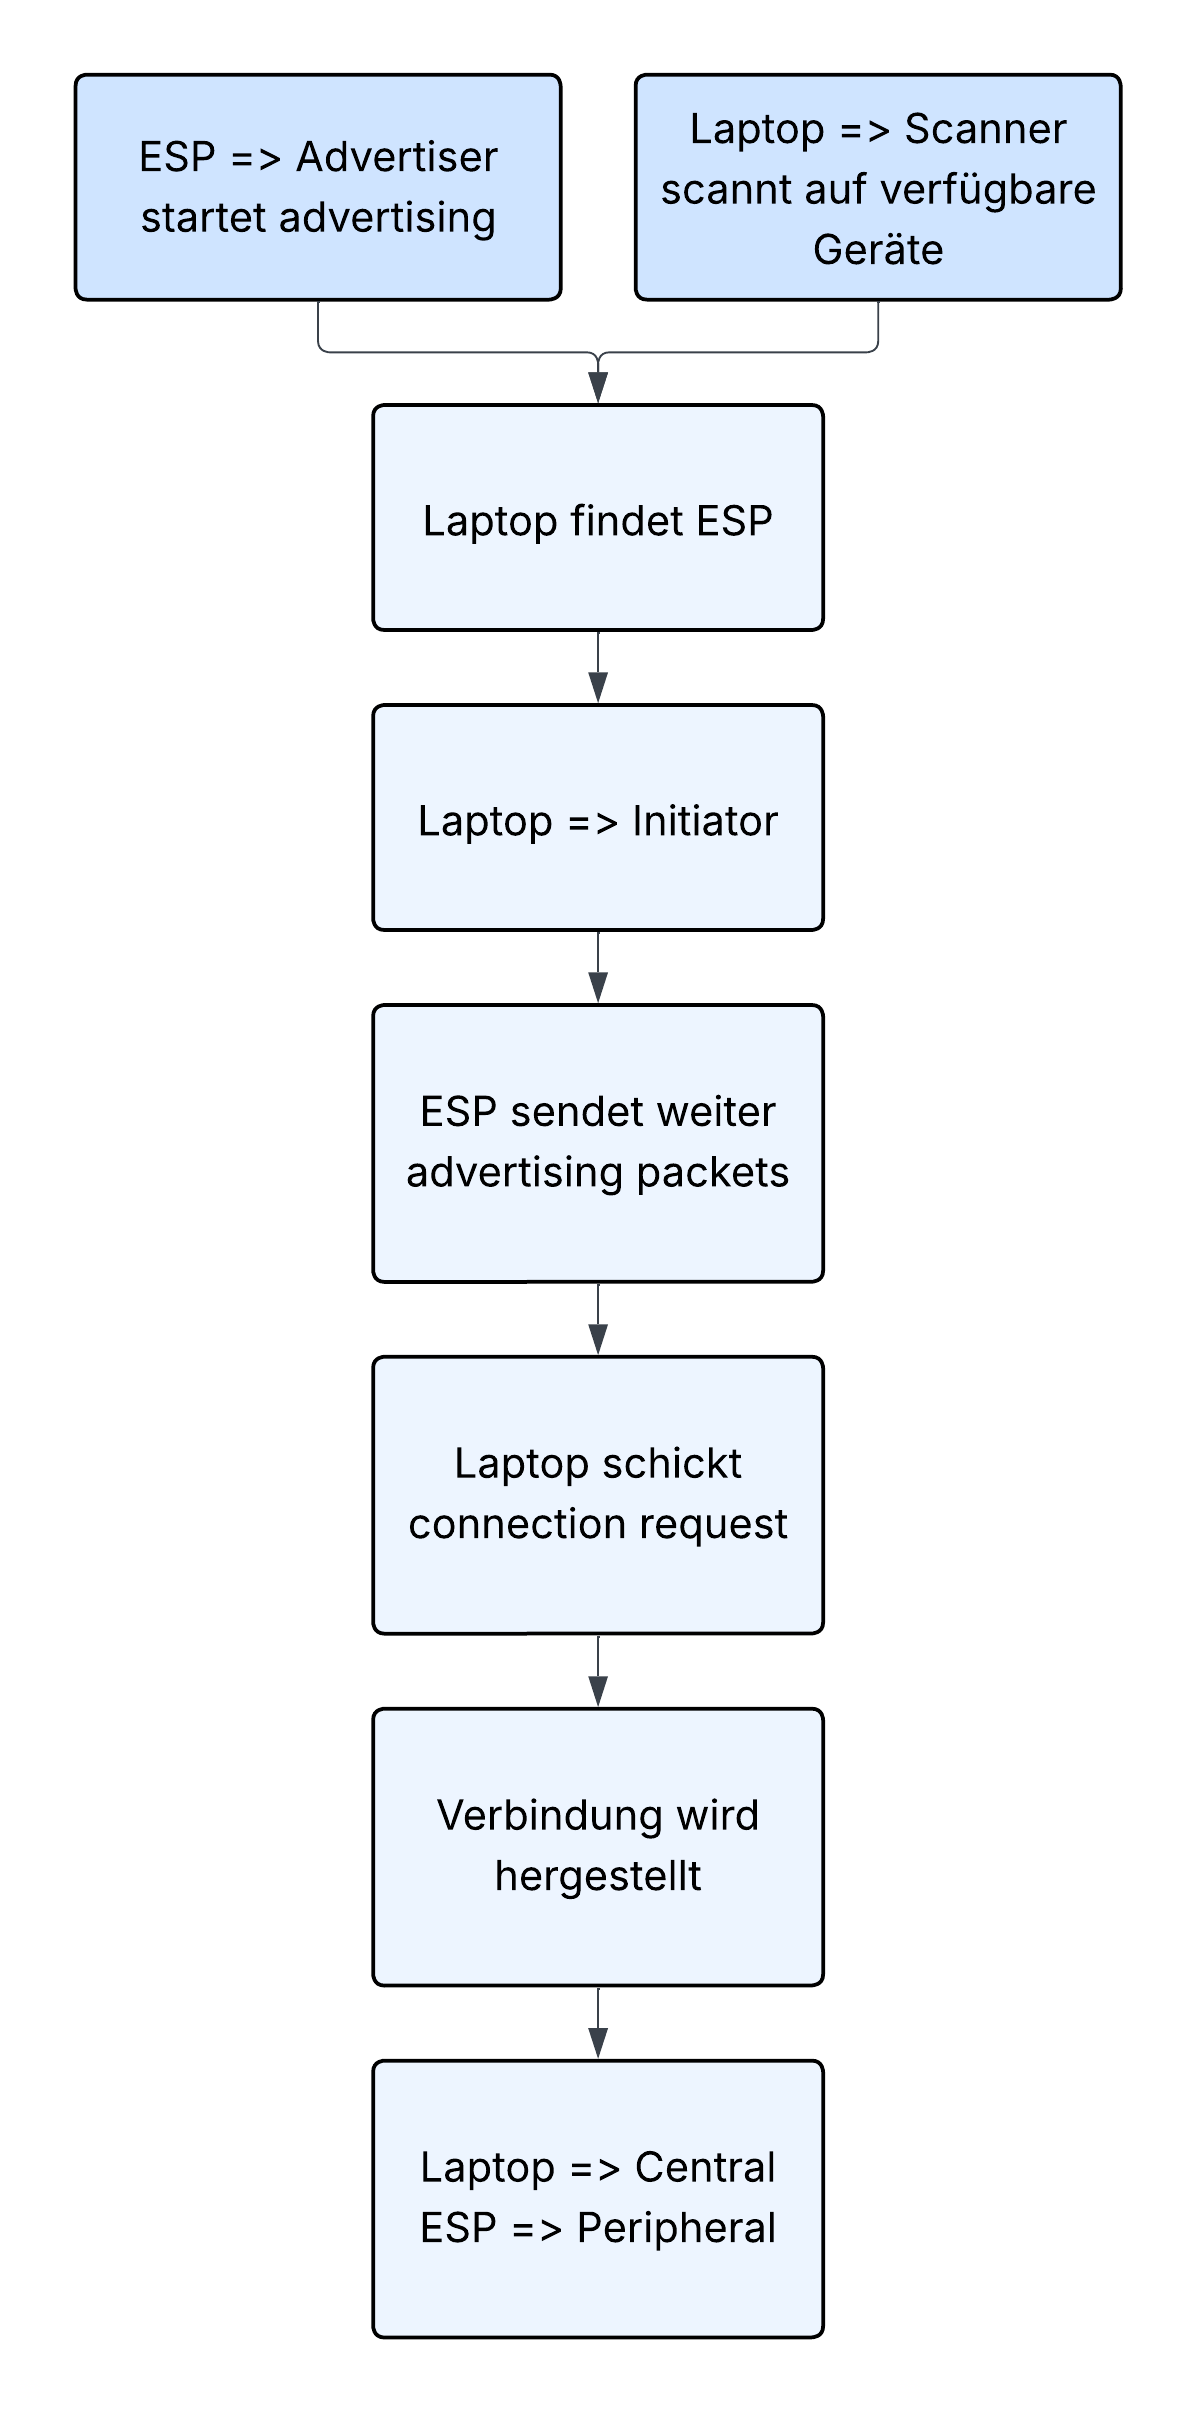
\includegraphics[width = 6cm]{images/ble-gap_bsp.png}
\caption{GAP Verbindungsaufbau}
\label{fig:ble_gap_bsp}
\end{figure}


\subsubsection{GATT (Generic Attribute Profile)}
Dieses Protokoll basiert auf einer hierarchischen Einteilung von Characteristic, Service und Profile. Hier legt der Benutzter eine Anwendung anhand der vorgegebenen Struktur von BLE an. Diese wird in der ATT Layer technisch umgesetzt und gespeichert. siehe \ref{ATT}.

\noindent
Characteristics sind Datenstrukturen die mit Attributen aufgebaut sind. Sie müssen ein Characteristic Declaration Attribute und ein Characteristic Value Attribute beinhalten. Optional gibt es die Möglichkeit noch weitere Descriptor Attributes in einer Characteristic zu implementieren.

\noindent
Services sind ebenfalls mit Attributen aufgebaut. Ein sogennates Service Declaration Attribute muss definiert sein. In einem Service sind mehrere Characteristics mit einer ähnlichen Funktion oder zusammenhängenden Funktionen gesammelt.

\noindent
Profiles sind die übergeordnetesten Instanzen. Sie müssen gewisse Services haben muss um einen Standard zu erfüllen. Bei der Verwendung von BLE werden sie im Programmcode nicht definiert, wie Characteristics und Services. Ein Profile entsteht in dieser Hinsicht in einem Projekt nur konzeptionell. \cite{espressif_ble_intro}



\subsubsection{ATT (Attribute Protocol)} \label{ATT}
Auf dieser Ebene passiert die technische Umsetzung des GATT. Eine dort erzeugt Charakteristik wird am Server Device als Attribute gespeichert. Attribute sind strukturiert in Type, Value und Permission. Dabei werden sie im Speicher meist als Arrays angelegt- Attribute Table. Der Type eines Attributs ist ein 32- oder öfter benutzte 128bit langer UUID (Universally Unique IDentifier). \cite{espressif_ble_intro}

\subsubsection{L2CAP (Logic Link Control and Adaption Layer Protocol)}
L2CAP ist für die Datenpaketverwaltung zuständig. Es wird auf Client- sowie auf Hostseite benutzt. Zu den Aufgaben gehören unter anderem Multiplexing, Segementierung und Wiederzusammensetzung der Daten. \cite{ti_ble_l2cap}

\subsubsection{SMP (Security Manager Protocol )}
Ist das Sicherheitsprotokoll von BLE, es ist ein Untermodul von GAP. \cite{espressif_bluetooth_security}



%\subsection{JLC ?}

\subsection{Realtime System}

\subsection{Bewegungssimulation}
%Motortheorie
%Vergleich Stepper vs. Servo

\subsection{Geräuschsimulation}
%Modul erklären
%Lautsprecher Theorie

\subsection{Wärmesimulation}
\subsubsection{Keramikwiderstände}


%PT100 Regelung? das was mc geyappt hat
%Keramikwiderstände vs. Heizelemente



\section{Platinendesign}
\subsection{KiCad}
%3d model



\section{3D Druck}


